% ==============================================================================
\section{Statistical Inference}%
\label{sec:statistical_inference}
% ==============================================================================

Techniques of statistical inference commonly used at the ATLAS experiment for
the interpretation of results of searches and measurements are introduced in the
following. Among these are methods for parameter estimation and hypothesis
testing. They are used to fit statistical models to observed data (or
pseudodata) and to make frequentist statements about the presence or absence of
a signal.


\subsection{The \textsc{HistFactory} Model}%
\label{sec:histfactory}

In high-energy physics, the use of binned data--usually in the form of
histograms--is widespread for visualisation and statistical modelling. Analyses
of collider data typically consider multiple mutually disjoint regions, also
referred to as \emph{channels}, defined by event selections. Each region
consists of one or more bins given by a discriminating variable. Events from
different signal and background processes, hereafter referred to as
\emph{physics processes}, contribute to these regions. In this context,
\textsc{HistFactory}~\cite{cranmer2012} is the tool used in this thesis to
construct statistical models for likelihood-based inference. The
\textsc{HistFactory} model is introduced in the following, adopting the notation
of Ref.~\cite{cranmer2012} with few modifications.

Let $\mathcal{C}$ denote the set of channels and $\mathcal{B}_{c}$ the set of
bins in channel~$c$. The probability of observing $n_{cb}$ events in bin~$b$ of
channel~$c$ is modelled by a Poisson distribution with probability mass function
$\pois(n_{cb} \mid \nu_{cb})$, where $\nu_{cb}$ denotes the expected number of
events for the given bin. The expectation~$\nu_{cb}$, which has to be inferred
from the observed data, is parameterised as
\begin{align*}
  \nu_{cb}(\myvec{\alpha}, \myvec{\phi}, \myvec{\gamma}) =
  \sum_{s \in \mathcal{S}_{c}} \, \gamma_{csb} \, \Phi_{cs}(\myvec{\phi}) \, \eta_{cs}(\myvec{\alpha}) \, \sigma_{csb}(\myvec{\alpha}) \,\text{,}
\end{align*}
where $\mathcal{S}_{c}$ is the set of physics processes contributing to
channel~$c$, and the parameters of the model are denoted by
${\myvec{\alpha} = (\alpha_1, \dots, \alpha_n)}$,
${\myvec{\phi} = (\phi_1, \dots, \phi_m)}$, and
$\myvec{\gamma}$~\cite{cranmer2012}.\footnote{The vector $\myvec{\gamma}$ groups
  the $\gamma_{csb}$ parameters for all bins.} Of these parameters,
$\myvec{\alpha}$ and $\myvec{\gamma}$ are nuisance parameters (NPs) with
external constraints, which will be introduced shortly.  The relevance of the
four factors $\gamma_{csb}$, $\Phi_{cs}$, $\eta_{cs}$, and $\sigma_{csb}$ is
described in the following~\cite{cranmer2012}:
\begin{itemize}

\item $\sigma_{csb}(\myvec{\alpha})$ is referred to as the \emph{parameterised
    histogram} of process~$s$ in channel~$c$, the index $b$ denoting the bins of
  the histogram. It serves to estimate the expected number of events from
  process~$s$ in channel~$c$ and is usually derived using simulation or control
  region data. The parameterised histogram has additional degrees of freedom,
  parameterised by $\myvec{\alpha}$, to account for uncertainties on the shape
  of the histogram. These degrees of freedom leave the overall normalisation
  $\sum_{b \in \mathcal{B}_{c}} \sigma_{csb}(\myvec{\alpha})$ for a given
  channel~$c$ and process~$s$ unchanged.

\item $\eta_{cs}(\myvec{\alpha})$ represents a normalisation factor applied
  uniformly to all bins of the parameterised histogram for a given process~$s$
  in channel~$c$. The normalisation factor $\eta_{cs}$ cannot vary freely, since
  it is a function of the constrained parameters $\myvec{\alpha}$. This factor
  is included to account for uncertainties on the normalisation of process~$s$
  in channel~$c$.

\item $\Phi_{cs}(\myvec{\phi})$ also represents a normalisation factor applied
  uniformly to all bins of the parameterised histogram for a given process~$s$
  in channel~$c$. However, $\Phi_{cs}$ is the product of \emph{free}
  (unconstrained) normalisation factors given by
  \begin{align*}
    \Phi_{cs}(\myvec{\phi}) = \prod_{p \in \mathcal{N}_{cs}} \phi_p \,\text{,}
  \end{align*}
  where $\mathcal{N}_{cs}$ denotes the set of indices that defines which
  normalisation factors are to be applied to a given process~$s$ in channel~$c$.
  % These parameters are optional, i.e.\ they can be fixed to unity for a given
  % process/channel depending on the statistical model one wants to construct.
  % % Normalisation factors that are shared?
  In most cases, at least one normalisation factor is present that is applied to
  the physics process of interest, also referred to as the \emph{signal}. This
  normalisation factor is referred to as the \emph{signal strength}~$\mu$ and is
  often considered to be the parameter of interest (POI). Normalisation factors
  are considered to be NPs if they are not POIs.

\item $\gamma_{csb}$ are parameters that introduce additional degrees of freedom
  for every bin. They are used to incorporate uncertainties that originate from
  sources that are independent between bins. An example of such an uncertainty
  is the statistical uncertainty arising from the use of finite samples of
  events to estimate $\sigma_{csb}$.

  In this thesis, the method by Barlow and Beeston~\cite{barlow1993} is used to
  account for statistical uncertainties on the estimation of $\sigma_{csb}$. To
  reduce the number of parameters of the statistical model, the method is
  simplified as proposed in Ref.~\cite{conway2011} by only considering the
  statistical uncertainty on $\sum_{s \in \mathcal{S}_{c}} \sigma_{csb}$ for a
  given bin and channel. Consequently, the parameters $\gamma_{csb}$ can be
  replaced by $\gamma_{cb}$, omitting the dependence on the physics process.

\end{itemize}
A description of the exact functional form of $\sigma_{csb}(\myvec{\alpha})$ and
$\eta_{cs}(\myvec{\alpha})$ is omitted here but can be found in
Ref.~\cite{cranmer2012}. The likelihood function of the statistical model is
given by
\begin{align}
  L(\myvec{\alpha}, \myvec{\phi}, \myvec{\gamma}) = \Biggl[\,
  \prod_{c \in \mathcal{C}}
  \prod_{b \in \mathcal{B}_{c}}
  \pois\bigl( n_{cb} \mid \nu_{cb}(\myvec{\alpha}, \myvec{\phi}, \myvec{\gamma}) \bigr)
  \,\Biggr]
  \times L_{\text{ext}}(\myvec{\alpha}, \myvec{\gamma}) \,\text{,}
  \label{eq:likelihood_histfactory}
\end{align}
where $L_{\text{ext}}(\myvec{\alpha}, \myvec{\gamma})$ is the likelihood
function defining the external constraints on the NPs~$\myvec{\alpha}$ and
$\myvec{\gamma}$. The external constraints are defined by
\begin{align*}
  L_{\text{ext}}(\myvec{\alpha}, \myvec{\gamma}) =
  \Biggl[\, \prod_{p=1}^{n} f(a_p \mid \alpha_p)     \,\Biggr]
  \Biggl[\, \prod_{c \in \mathcal{C}} \prod_{b \in \mathcal{B}_{c}} \pois(m_{cb} \mid \gamma_{cb} \tau_{cb}) \,\Biggr] \,\text{,}
\end{align*}
with the terms in brackets being described in the following:
\begin{itemize}

\item The term $f(a_p \mid \alpha_p)$ can be interpreted as the likelihood
  function of an auxiliary measurement of the parameter~$\alpha_p$ given that
  $a_p$ is observed. Conventionally, $f(a_p \mid \alpha_p)$ is taken to be the
  probability density of a Normal distribution with unit variance and mean
  $\alpha_p$. Furthermore, it is assumed that the measurement observed $a_p = 0$
  such that, considering only the auxiliary measurement, the maximum likelihood
  estimate (MLE) of $\alpha_p$ is 0 with an uncertainty of
  $\Delta \alpha_p = \pm 1$. This particular choice of constraint term is
  closely connected to the functional form of $\sigma_{csb}(\myvec{\alpha})$ and
  $\eta_{cs}(\myvec{\alpha})$, i.e.\ for a single parameter $\sigma_{csb}(0)$
  and $\eta_{cs}(0)$ represent the nominal histogram and normalisation, while
  $\sigma_{csb}(\pm 1)$ and $\eta_{cs}(\pm 1)$ correspond to $\pm 1 \sigma$
  variations of the histogram shape and normalisation, respectively.

  % which completely describe the physical effects of the nuisance
  % parameter.\footnote{\cite{cranmer2012}.}

\item The $\pois(m_{cb} \mid \gamma_{cb} \tau_{cb})$ terms provide constraints
  for the $\gamma_{cb}$ parameters introduced by the (simplified)
  Barlow--Beeston method. For every bin a constant
  $ \tau_{cb} = ( \sum_i w_i )^2 / \sum_i w_i^2 $ is defined, where the
  summations go over all events making up the background prediction in the given
  bin and $w_i$ is the event weight of event~$i$. This constant is interpreted
  as an effective number of unweighted events,\footnote{Let
    $Y_{\text{w}} = \sum_{i = 1}^{N} W_i$ and
    $Y = \sum_{i = 1}^{N^\prime} 1 = N^\prime$, where $N$ and $N^\prime$ are
    independent Poisson random variables and $W_i$ are i.i.d.\ weights that are
    independent of $N$ and $N^\prime$. The effective number of unweighted events
    refers to the value of $\expect(N^\prime)$ that ensures that the relative
    standard deviation of $Y_{\text{w}}$ and $Y$ are equal. This condition
    yields $\expect(N^\prime) = \expect(N) \expect(W)^2 / \expect(W^2)$, and
    after approximating expected values with sample averages
    $\expect(N^\prime) \approx ( \sum_i w_i )^2 / \sum_i w_i^2$.} which is a
  measure of the statistical precision of the background estimate in the
  bin. This statistical uncertainty is incorporated in the model by setting up
  auxiliary measurements of the effective number of unweighted events,
  $\gamma_{cb}\tau_{cb}$, for every bin. These measurements are assumed to
  observe $m_{cb} = \tau_{cb}$, and therefore the nominal values of the
  $\gamma_{cb}$ parameters is 1.
\end{itemize}
% Once all parameters of the \textsc{HistFactory} model are fixed, the
% probability distributions of the observables~$n_{cb}$
%
% $n_{cb}$ ``observables''
%
% $a_p$ $m_{cb}$ ``global observables''

The parameters of the model can be estimated, given the observed data, using
maximum likelihood estimation. Hereafter, it is assumed that the model has one
POI denoted by $\mu$ that is to be interpreted as a signal strength. All other
(non-POI) parameters of the model are collectively referred to as
$\myvec{\theta}$. Let $\Omega$ be the parameter space of the model with
elements~$(\mu, \myvec{\theta})$. The MLE of the parameters are determined by
the \emph{unconditional fit}
\begin{align}
  (\muhat, \hat{\myvec{\theta}}) = \argmax_{(\mu, \myvec{\theta}) \in \Omega} L(\mu, \myvec{\theta}) \,\text{.}
  \label{eq:unconditional_fit}
\end{align}
Often, a restricted model is constructed by fixing the POI to an arbitrary value
$\mu^*$. In this case, the MLE of the model parameters are given by the
\emph{conditional fit for $\mu = \mu^*$}
\begin{align}
  \hat{\hat{\myvec{\theta}}}(\mu^*) = \argmax_{\myvec{\theta} \in \{ \myvec{\theta}^\prime \mid (\mu^\prime, \myvec{\theta}^\prime) \in \Omega \,\land\, \mu^\prime = \mu^* \} } L(\mu^*, \myvec{\theta}) \,\text{.}
  \label{eq:conditional_fit}
\end{align}
Hereafter, the model with the restriction $\mu = 0$ is referred to as the
\emph{background-only model}. The unrestricted model is referred to as the
\emph{signal-plus-background model}.

Lastly, special datasets referred to as \emph{Asimov
  datasets}~\cite{Cowan:2010js} are introduced. For a given set of model
parameters, the Asimov dataset is the dataset in which the observables $n_{cb}$
and the global observables $a_p$ and $m_{cb}$ are equal to their expected
values. Asimov datasets can be used, in place of the observed data, to evaluate
the expected experimental sensitivity of searches or measurements in HEP. Some
uses of Asimov datasets will be highlighted in the subsequent sections.


\subsection{Hypothesis Testing}%
\label{sec:hypotesting}

In high-energy physics, one is often concerned with comparing the goodness of
fit of competing statistical models to observed data. These comparisons allow to
make statements about values of the signal strength that are still in agreement
with the observations. The framework of \emph{statistical hypothesis testing}
provides a principled approach to perform these comparisons.

With the statistical model introduced previously, a null hypothesis, $H_0$, is
defined as
\begin{alignat*}{3}
  &H_0: (\mu, \myvec{\theta}) \in \Omega_0
    \quad &\text{with} \quad &\Omega_0 \subset \Omega \,\text{,} \\
  \intertext{where $\Omega_0$ is the set of model parameters that specify the
  null hypothesis, and an alternative hypothesis, $H_1$, is defined as}
  &H_1: (\mu, \myvec{\theta}) \in \Omega_1
    \quad &\text{with} \quad &\Omega_1 = \Omega \setminus \Omega_0 \,\text{.}
\end{alignat*}
% \begin{align*}
%   H_1: (\mu, \myvec{\theta}) \in \Omega_1
%   \quad \text{with} \quad \Omega_1 = \Omega \setminus \Omega_0 \,\text{.}
    %   \end{align*}
%
% \footnote{Example: Taking the background-only hypothesis as
%   the null hypothesis, then $\Omega_0 = \{ (\mu^\prime, \myvec{\theta}^\prime) \in \Omega \mid \mu^\prime = 0 \}$.}
%
A \emph{likelihood ratio test} (LRT) can be used to compare the hypotheses. The
test statistic of the LRT is given by
\begin{align*}
  \Lambda = -2 \ln\mathopen{}\left[
  \frac{\sup_{(\mu, \myvec{\theta}) \in \Omega_0} L(\mu, \myvec{\theta})}
  {\sup_{(\mu, \myvec{\theta}) \in \Omega\phantom{_0}} L(\mu, \myvec{\theta})}
  \right]\mathclose{} \,\text{,}
\end{align*}
where the numerator (denominator) of the term in brackets is the supremum of the
likelihood for the restricted (unrestricted) model~\cite{casella2001}. A
critical value of the test statistic, $\Lambda_{\text{crit}}$, is chosen and
compared to the observed value of the test statistic. If
$\Lambda > \Lambda_{\text{crit}}$ then $H_0$ is rejected in favour of
$H_1$. Otherwise, $H_0$ cannot be rejected. The chosen value of
$\Lambda_{\text{crit}}$ defines the rejection region of the test and thus its
statistical significance and power.


\subsubsection{Discovery of a Signal}

In the framework of hypothesis testing, the discovery of a signal implies
rejecting the background-only hypothesis in favour of the signal-plus-background
hypothesis. Usually, only signals with positive strength, that is $\mu > 0$, are
considered as potential discoveries. The relevant hypotheses for testing the
discovery of a signal are
\begin{align*}
  &H_0: (\mu, \myvec{\theta}) \in \{ (\mu^\prime, \myvec{\theta}^\prime) \in \Omega^+ \mid \mu^\prime = 0 \}
  &&H_1: (\mu, \myvec{\theta}) \in \{ (\mu^\prime, \myvec{\theta}^\prime) \in \Omega^+ \mid \mu^\prime > 0 \} \,\text{,}
\end{align*}
where $\Omega^+$ denotes the parameter space of the model with the restriction
that $\mu \geq 0$. An empirical test statistic based on the LRT is defined as
\begin{align*}
  q_0 = \begin{cases}
          -2 \ln\mathopen{}\left[ \frac{ L\bigl(0, \hat{\hat{\myvec{\theta}}}(0) \bigr)}{L\bigl( \muhat, \hat{\myvec{\theta}} \bigr)} \right]\mathclose{}, & \muhat > 0 \\
          0,          & \muhat \leq 0
        \end{cases} \quad\text{,}
\end{align*}
where $\muhat$, $\hat{\myvec{\theta}}$, and $\hat{\hat{\myvec{\theta}}}$ are
defined as in
\Cref{eq:unconditional_fit,eq:conditional_fit}~\cite{Cowan:2010js}.\footnote{The
  unconditional fit is performed without the $\mu \geq 0$ constraint. Instead,
  the constraint is imposed in the definition of the test statistic by setting
  the maximum likelihood of the unrestricted model to
  $L\bigl( 0, \hat{\hat{\myvec{\theta}}}(0) \bigr)$ in the $\muhat < 0$ case.}
This test statistic is referred to as the \emph{discovery test statistic}. The
asymptotic sampling distribution of $q_0$ under $H_0$ is given by the
probability density function
\begin{align*}
  f(q_0) = \frac{1}{2} \delta(q_0) + \frac{1}{2} f_{\chi^2}(q_0; 1) \,\text{,}
\end{align*}
which is an equal mixture of a Dirac $\delta$ distribution and a $\chi^2$
distribution with one degree of freedom~\cite{Cowan:2010js}. The discovery test
statistic is often expressed in terms of an asymptotic $p$-value according
to
\begin{align*}
  p_0 = \int_{q_{0}}^\infty \mathrm{d}q_0^\prime \, f(q_0^\prime) =
  1 - \Phi\left(\sqrt{q_{0}}\right) \,\text{,}
\end{align*}
where $\Phi$ is the cumulative distribution function of the Standard Normal
distribution~\cite{Cowan:2010js}. Another way of expressing the test statistic
is in terms of the \emph{discovery significance}~$Z_0$, which is defined
as~\cite{Cowan:2010js}
\begin{align*}
  Z_0 = \Phi^{-1}(1 - p_0) = \sqrt{q_{0}} \,\text{.}
\end{align*}
In particle physics, the conventional significance threshold that has to be
exceeded to claim discovery of new physics is $Z_0 = 5$ ($p_0 = \num{2.87e-7}$),
which is also referred to as the ``$5\sigma$ threshold''. Lastly, the
\emph{median discovery significance} of a signal with an assumed strength of
$\mu$ can be estimated by using an Asimov dataset with the same signal strength
in the determination of $Z_0$~\cite{Cowan:2010js}. The median discovery
significance is also referred to as the \emph{expected signal significance}.

\subsubsection{Upper Limits on the Signal Strength}

Often, one is interested in determining the largest signal strength that would
still be compatible with the observed data. Formally, this constitutes
estimating a one-sided confidence interval for $\mu$ that is bounded from above,
hence referred to as an upper limit. The upper limit can be obtained by
inverting a test of the hypotheses
\begin{align*}
  &H_0: (\mu, \myvec{\theta}) \in \{ (\mu^\prime, \myvec{\theta}^\prime) \in \Omega^+ \mid \mu^\prime \geq \mu^* \}
  &&H_1: (\mu, \myvec{\theta}) \in \{ (\mu^\prime, \myvec{\theta}^\prime) \in \Omega^+ \mid \mu^\prime < \mu^* \} \,\text{,}
\end{align*}
where $\mu^*$ is used to parameterise the hypotheses. Let $(1 - \alpha)$ be the
desired confidence level (CL) of the interval to be estimated. Given a test of
$H_0$ and $H_1$ with significance level~$\alpha$, the confidence interval is the
set of values of $\mu^*$ for which $H_0$ cannot be rejected by the test. The
upper bound of this set is referred to as the upper limit on $\mu$ at
$(1 - \alpha)$~CL. The estimation of upper limits in HEP uses an empirical test
statistic derived from the LRT that reads
\begin{align*}
  \qmutilde =
  \begin{cases}
    -2\ln\mathopen{}\left[ \frac{ L\bigl( \mu, \hat{\hat{\myvec{\theta}}}(\mu) \bigr)}{L\bigl( 0, \hat{\hat{\myvec{\theta}}}(0) \bigr)} \right]\mathclose{}, & \muhat \in (\infty, 0] \\[1em]
    -2\ln\mathopen{}\left[ \frac{ L\bigl( \mu, \hat{\hat{\myvec{\theta}}}(\mu) \bigr)}{L\bigl( \muhat, \hat{\myvec{\theta}} \bigr)} \right]\mathclose{}, & \muhat \in (0, \mu] \\[1em]
    0,\phantom{ \biggl[  \biggr]} & \muhat \in (\mu, \infty) \\
  \end{cases} \,\text{,}
\end{align*}
where for notational simplicity $\mu^*$ is denoted as
$\mu$~\cite{Cowan:2010js}. The asymptotic sampling distributions of \qmutilde
were derived in Ref.~\cite{Cowan:2010js} for any assumed value of the true
signal strength. Let~$f(\qmutilde \mid \mu^\prime)$ be the asymptotic sampling
distribution of \qmutilde under the assumption that the signal strength is
$\mu^\prime$. Following the approach outlined before, an approximate upper limit
at $(1 - \alpha)$~CL can be determined by finding the largest $\mu$ such that
\begin{align*}
  p_\mu = \int_{\tilde{q}_{\mu, \text{obs}}}^{\infty} \mathrm{d}\qmutilde \, f(\qmutilde \mid \mu) \leq \alpha \,\text{,}
\end{align*}
where $\tilde{q}_{\mu, \text{obs}}$ denotes the observed value of the test
statistic.

In searches for new physics, a modified approach referred to as the
\CLs~technique~\cite{Junk:1999kv,Read:2002hq} is adopted to derive upper limits
on $\mu$. The method of estimating upper limits based on $p_\mu$ is susceptible
to setting overly stringent constraints on $\mu$ in regions with little signal
sensitivity. While this is expected given a coverage probability below
\SI{100}{\percent}, it is preferred to avoid the spurious exclusion of signals
in regions with no sensitivity. This problem is addressed by the \CLs method
which introduces a modified test statistic defined as
\begin{align}
  \CLs = \frac
  {\int_{\tilde{q}_{\mu, \text{obs}}}^{\infty} \mathrm{d}\qmutilde \, f(\qmutilde \mid \mu)}
  {\int_{\tilde{q}_{\mu, \text{obs}}}^\infty \mathrm{d}\qmutilde \, f(\qmutilde \mid 0)} \,\text{.}
  \label{eq:cls}
\end{align}
The \CLs statistic modifies $p_\mu$ (the numerator) by dividing it by the power
of the \qmutilde-based test in rejecting $H_0$ when the background-only
hypothesis is true. This modification can be understood qualitatively by
considering two edge cases:
\begin{itemize}

\item High signal sensitivity: the power of the test to reject $H_0$ under the
  background-only hypothesis approaches unity and thus $\CLs \approx p_\mu$.

\item Low signal sensitivity: the power of the test to reject $H_0$ under the
  background-only hypothesis approaches $p_\mu$ and thus $\CLs \approx 1$.

\end{itemize}
A graphical illustration of these cases is given in \Cref{fig:cls_qmutilde}.

\begin{figure}[htbp]
  \centering

  \begin{subfigure}{0.46\textwidth}
    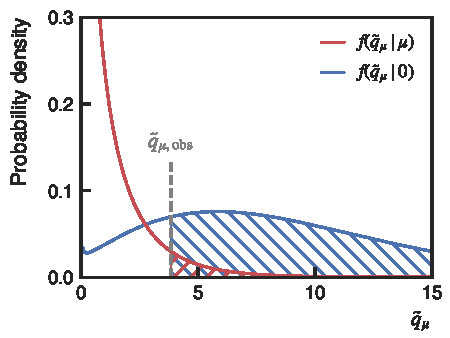
\includegraphics[width=\textwidth]{statistics/cls_high_sensitivity}
    \caption{Example with high signal sensitivity}
  \end{subfigure}\hfill%
  \begin{subfigure}{0.46\textwidth}
    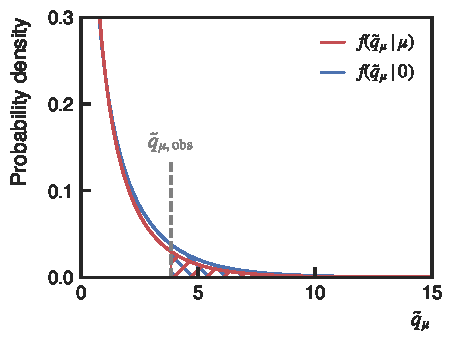
\includegraphics[width=\textwidth]{statistics/cls_low_sensitivity}
    \caption{Example with low signal sensitivity}
  \end{subfigure}

  \caption{Qualitative illustration of the sampling distributions of \qmutilde
    under the signal-plus-background (red) and background-only (blue)
    hypothesis. The red (blue) hatched area corresponds to the integrals
    entering the numerator (denominator) of the \CLs statistic
    in~\Cref{eq:cls}.}%
  \label{fig:cls_qmutilde}
\end{figure}

Upper limits on $\mu$ using the \CLs technique are estimated by finding the
largest value of $\mu$ for which $\CLs \leq \alpha$. Since \CLs approaches unity
in cases of low signal sensitivity, spurious exclusions of signals are
effectively prevented. Upper limits derived from the condition
$\CLs \leq \alpha$ are also referred to as upper limits at $(1 - \alpha)$~CL,
however, these limits have to be interpreted as being conservative in the sense
that the coverage probability of the estimated intervals exceeds $(1 - \alpha)$
by construction due to $\CLs \geq p_\mu$. Conventionally, upper limits are set
at $\SI{95}{\percent}$~CL ($\alpha = 0.05$) in HEP. Hereafter, all quoted upper
limits are estimated using the \CLs technique. Finally, median upper limits on
$\mu$--also referred to as expected upper limits--can be derived by performing
the procedure outlined above using background-only Asimov datasets instead of
the observed data~\cite{Cowan:2010js}.


%%% Local Variables:
%%% mode: latex
%%% TeX-master: "../../phd_thesis"
%%% End:
